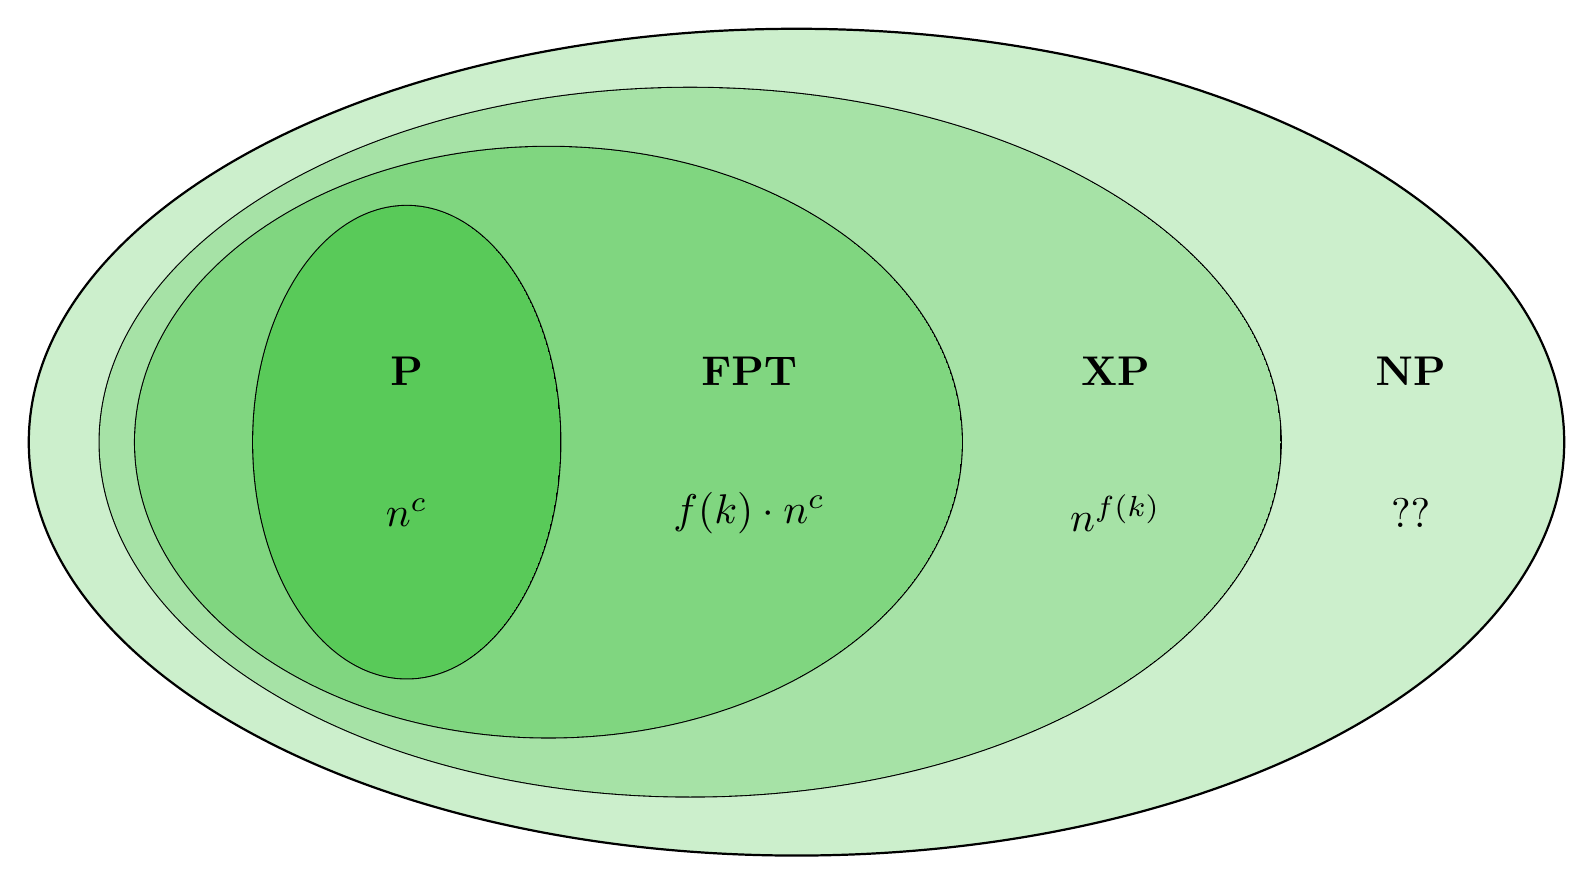
\begin{tikzpicture}[scale=1.5, transform shape,font=\normalsize]
	\colorlet{fillcolor}{black!32!green}
	\draw[thick,fill=fillcolor!20] (3.3,0) ellipse (6.5 and 3.5);
	\scope
		\draw[thick] (2.4,0) ellipse (5 and 3);
		\clip (2.4,0) ellipse (5 and 3);
		\fill[fillcolor!35] (2.4,0) ellipse (5 and 3);
		\scope
			\draw[thick] (1.2,0) ellipse (3.5 and 2.5);
			\clip (1.2,0) ellipse (3.5 and 2.5);
			\fill[fillcolor!50] (1.2,0) ellipse (3.5 and 2.5);
			\scope
				\draw[thick] (0,0) ellipse (1.3 and 2);
				\clip (0,0) ellipse (1.3 and 2);
				\fill[fillcolor!65] (0,0) ellipse (1.3 and 2);
			\endscope
		\endscope
	\endscope



	%labels
	\node at (0.0,0.6) {\bf P};
	\node at (2.9,0.6) {\bf FPT};
	\node at (6.0,0.6) {\bf XP};
	\node at (8.5,0.6) {\bf NP};

	\node at (0.0,-0.6) {$n^c$};
	\node at (2.9,-0.6) {$f(k)\cdot n^c$};
	\node at (6.0,-0.6) {$n^{f(k)}$};
	\node at (8.5,-0.6) {??};
\end{tikzpicture}
